% ==============================================================================
% Proyecto:     HPicoRV32 (Hardened PicoRV32)
% Archivo:      docs/arch/tmr_pc_rtl.tex
% Descripción:  Esquema RTL interno de PicoRV32 con triplicación TMR, votador
%               mayoritario 2-de-3, detección XOR y lazo Self-Healing en 1 ciclo
%               Colores xcolor estándar y coordenadas centradas para Oleafly
% Compilación:  pdflatex tmr_pc_rtl.tex  (o incluir figures/tmr_pc_rtl.tikz)
% ==============================================================================
\documentclass[tikz,border=14pt]{standalone}

\usepackage[utf8]{inputenc}
\usepackage[T1]{fontenc}
\usepackage{helvet}
\renewcommand{\familydefault}{\sfdefault}

\usepackage{tikz}
\usetikzlibrary{arrows.meta}

\begin{document}
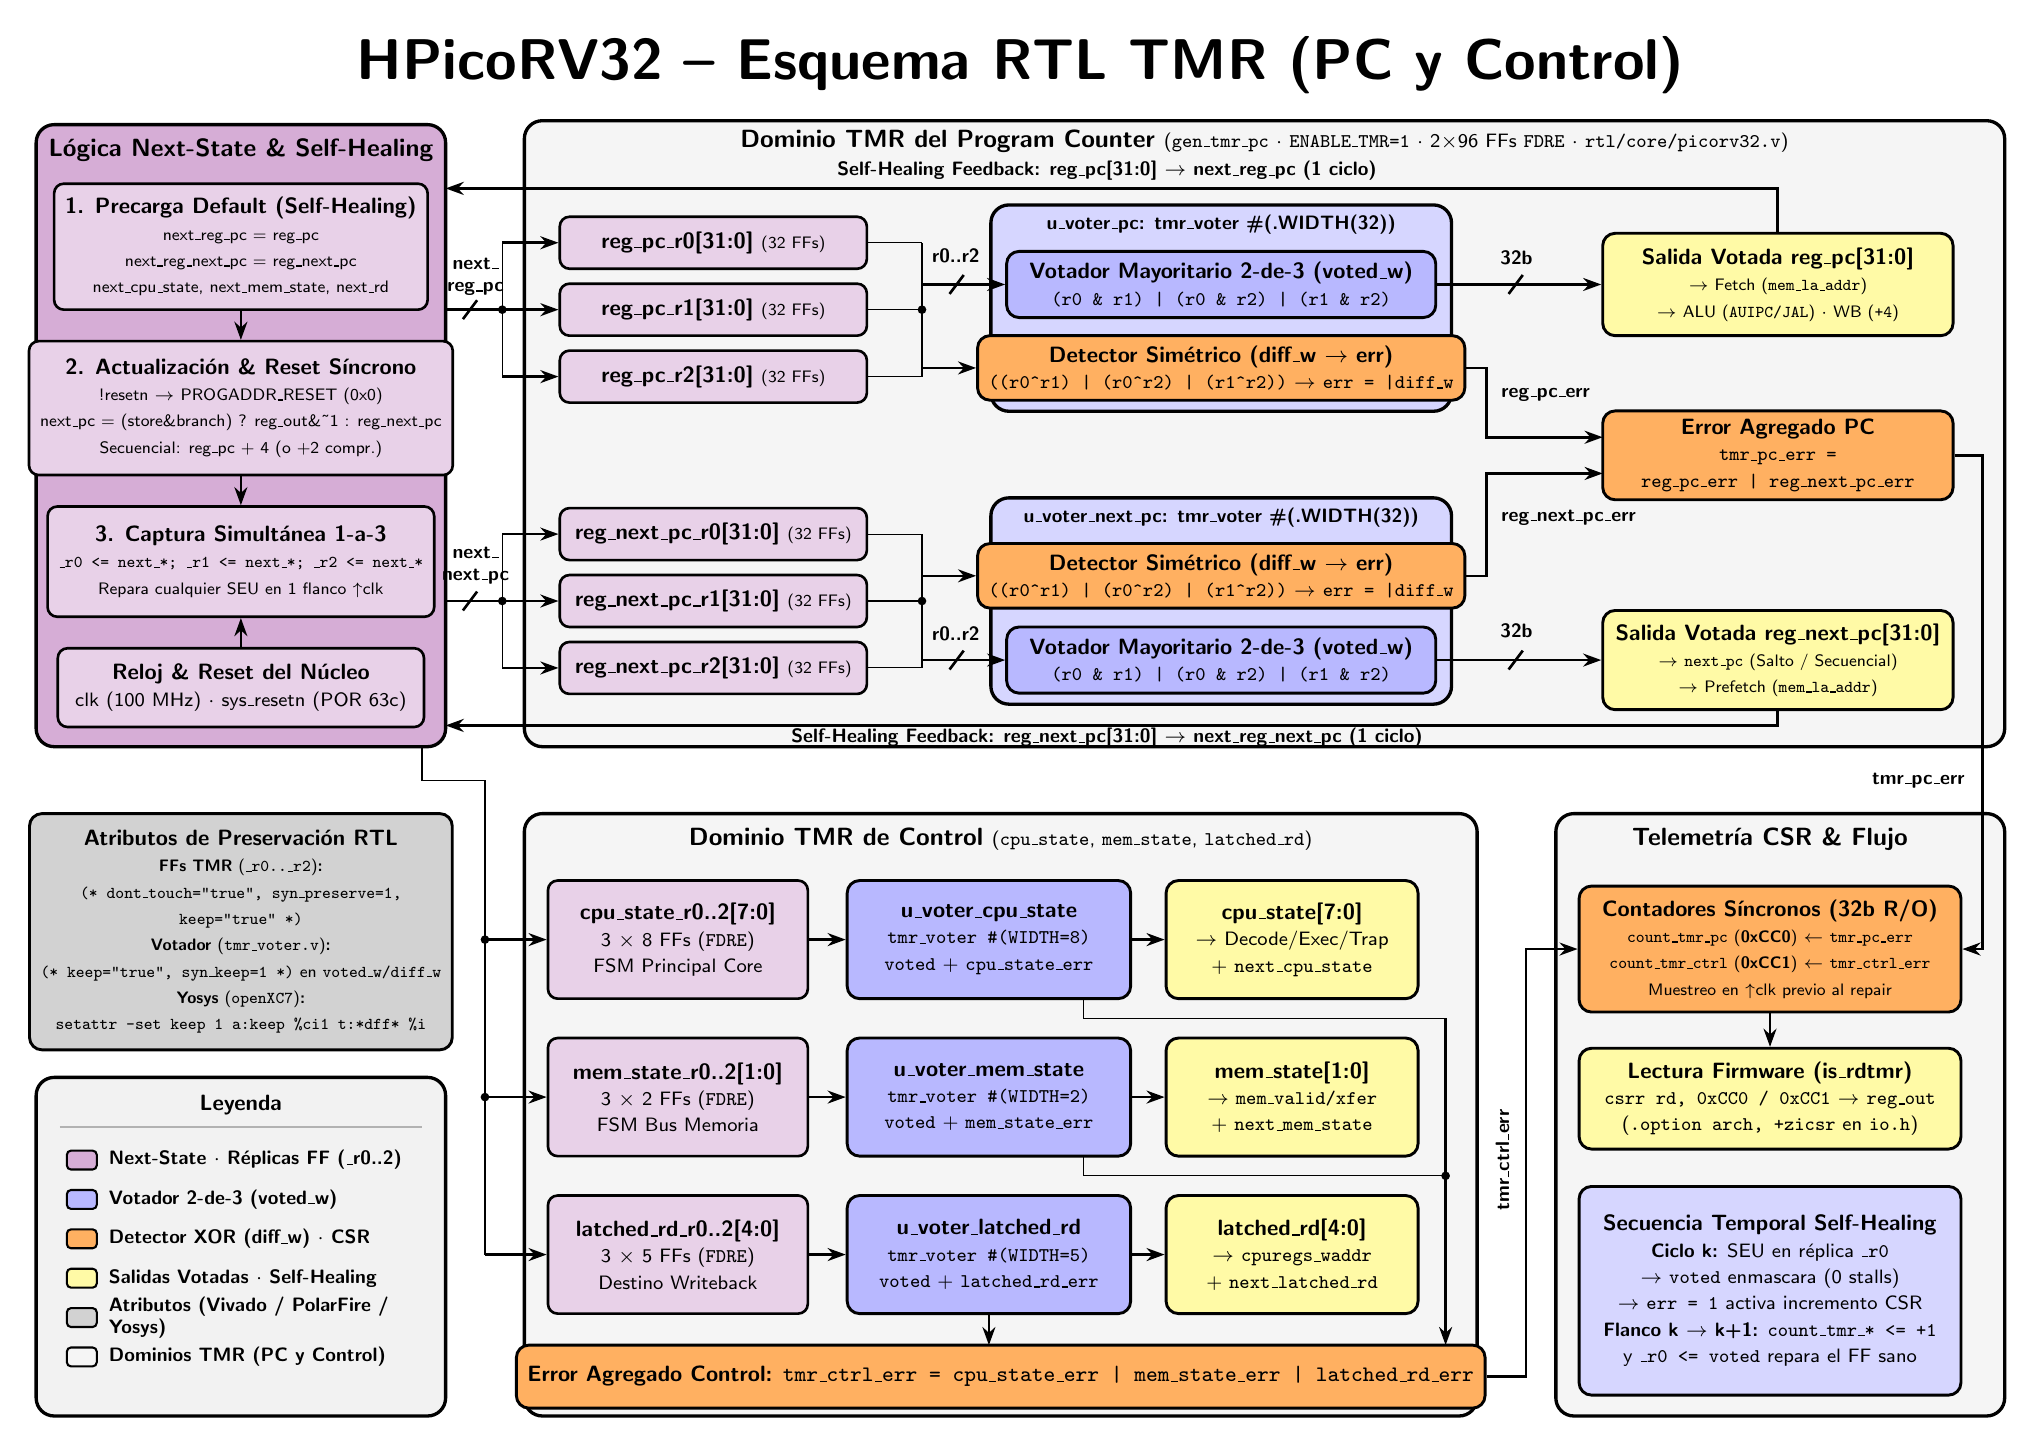
\begin{tikzpicture}[
  >= {Stealth[length=2.3mm, width=1.65mm]},
  blk/.style={
    draw=black,
    line width=1.05pt,
    rounded corners=4.5pt,
    align=center,
    text=black,
    font=\footnotesize,
    inner xsep=4pt,
    inner ysep=3pt
  },
  subblk/.style={
    draw=black,
    line width=0.95pt,
    rounded corners=3.5pt,
    align=center,
    text=black,
    font=\footnotesize,
    inner xsep=4pt,
    inner ysep=2.5pt
  },
  container/.style={
    draw=black,
    line width=1.2pt,
    rounded corners=6.5pt,
    inner sep=0pt
  },
  swatch/.style={
    draw=black,
    line width=0.75pt,
    rounded corners=1.5pt,
    inner sep=0pt,
    minimum width=0.38cm,
    minimum height=0.24cm
  },
  sig/.style={
    ->,
    draw=black,
    line width=0.95pt
  },
  bisig/.style={
    <->,
    draw=black,
    line width=0.95pt
  },
  tick/.style={
    draw=black,
    line width=0.95pt
  },
  lbl/.style={
    font=\scriptsize\bfseries,
    text=black,
    inner sep=1.5pt
  }
]

% ==============================================================================
% 0. Cabecera
% ==============================================================================
\node[font=\huge\bfseries] at (12.50, 17.90)
  {HPicoRV32 -- Esquema RTL TMR (PC y Control)};

% ==============================================================================
% 1. Columna Izquierda: Lógica Next-State / Self-Healing + Atributos + Leyenda
% ==============================================================================

% --- Contenedor Lógica Next-State & Self-Healing (always @(posedge clk)) ---
\node[container, fill=violet!32, minimum width=5.20cm, minimum height=7.90cm]
  (next_box) at (2.60, 13.20) {};
\node[font=\small\bfseries] at (2.60, 16.82)
  {Lógica Next-State \& Self-Healing};

\node[subblk, fill=violet!18, minimum width=4.65cm, minimum height=1.60cm]
  (preload_blk) at (2.60, 15.60)
  {\textbf{1. Precarga Default (Self-Healing)}\\\fontsize{6.3}{7.8}\selectfont next\_reg\_pc = reg\_pc\\\fontsize{6.3}{7.8}\selectfont next\_reg\_next\_pc = reg\_next\_pc\\\fontsize{6.3}{7.8}\selectfont next\_cpu\_state, next\_mem\_state, next\_rd};

\node[subblk, fill=violet!18, minimum width=4.65cm, minimum height=1.70cm]
  (update_blk) at (2.60, 13.55)
  {\textbf{2. Actualización \& Reset Síncrono}\\\fontsize{6.3}{7.8}\selectfont !resetn $\rightarrow$ PROGADDR\_RESET (0x0)\\\fontsize{6.3}{7.8}\selectfont next\_pc = (store\&branch) ? reg\_out\&\~{}1 : reg\_next\_pc\\\fontsize{6.3}{7.8}\selectfont Secuencial: reg\_pc + 4 (o +2 compr.)};

\node[subblk, fill=violet!18, minimum width=4.65cm, minimum height=1.40cm]
  (write_blk) at (2.60, 11.60)
  {\textbf{3. Captura Simultánea 1-a-3}\\\fontsize{6.3}{7.8}\selectfont \texttt{\_r0 <= next\_*; \_r1 <= next\_*; \_r2 <= next\_*}\\\fontsize{6.3}{7.8}\selectfont Repara cualquier SEU en 1 flanco $\uparrow$clk};

\node[subblk, fill=violet!18, minimum width=4.65cm, minimum height=1.00cm]
  (clkrst_blk) at (2.60, 10.00)
  {\textbf{Reloj \& Reset del Núcleo}\\\scriptsize clk (100 MHz) $\cdot$ sys\_resetn (POR 63c)};

\draw[sig] (preload_blk.south) -- (update_blk.north);
\draw[sig] (update_blk.south) -- (write_blk.north);
\draw[sig] (clkrst_blk.north) -- (write_blk.south);

% --- Atributos de Síntesis Multi-Herramienta ---
\node[blk, fill=gray!35, minimum width=5.20cm, minimum height=3.00cm]
  (attr_blk) at (2.60, 6.90)
  {\textbf{Atributos de Preservación RTL}\\\fontsize{6.2}{7.6}\selectfont \textbf{FFs TMR} (\texttt{\_r0..\_r2})\textbf{:}\\\fontsize{5.6}{6.9}\selectfont \texttt{(* dont\_touch="true", syn\_preserve=1,}\\\fontsize{5.6}{6.9}\selectfont \texttt{keep="true" *)}\\\fontsize{6.2}{7.6}\selectfont \textbf{Votador} (\texttt{tmr\_voter.v})\textbf{:}\\\fontsize{5.6}{6.9}\selectfont \texttt{(* keep="true", syn\_keep=1 *)} en \texttt{voted\_w/diff\_w}\\\fontsize{6.2}{7.6}\selectfont \textbf{Yosys} (\texttt{openXC7})\textbf{:}\\\fontsize{5.6}{6.9}\selectfont \texttt{setattr -set keep 1 a:keep \%ci1 t:*dff* \%i}};

% --- Leyenda ---
\node[container, fill=gray!10, minimum width=5.20cm, minimum height=4.30cm]
  (leyenda_box) at (2.60, 2.90) {};
\node[font=\footnotesize\bfseries] at (2.60, 4.70)
  {Leyenda};
\draw[line width=0.6pt, gray!60] (0.30, 4.42) -- (4.90, 4.42);

\node[swatch, fill=violet!32] (sw_ff) at (0.58, 4.00) {};
\node[font=\scriptsize\bfseries, text width=3.95cm, align=left] at (2.90, 4.00) {Next-State $\cdot$ Réplicas FF (\_r0..2)};

\node[swatch, fill=blue!28] (sw_vot) at (0.58, 3.50) {};
\node[font=\scriptsize\bfseries, text width=3.95cm, align=left] at (2.90, 3.50) {Votador 2-de-3 (voted\_w)};

\node[swatch, fill=orange!62] (sw_err) at (0.58, 3.00) {};
\node[font=\scriptsize\bfseries, text width=3.95cm, align=left] at (2.90, 3.00) {Detector XOR (diff\_w) $\cdot$ CSR};

\node[swatch, fill=yellow!35] (sw_out) at (0.58, 2.50) {};
\node[font=\scriptsize\bfseries, text width=3.95cm, align=left] at (2.90, 2.50) {Salidas Votadas $\cdot$ Self-Healing};

\node[swatch, fill=gray!35] (sw_attr) at (0.58, 2.00) {};
\node[font=\scriptsize\bfseries, text width=3.95cm, align=left] at (2.90, 2.00) {Atributos (Vivado / PolarFire / Yosys)};

\node[swatch, fill=gray!8] (sw_dom) at (0.58, 1.50) {};
\node[font=\scriptsize\bfseries, text width=3.95cm, align=left] at (2.90, 1.50) {Dominios TMR (PC y Control)};

% ==============================================================================
% 2. Contenedor Principal Superior Derecho: Dominio TMR del Program Counter
% ==============================================================================
\node[container, fill=gray!8, minimum width=18.80cm, minimum height=7.95cm]
  (pc_dom_box) at (15.60, 13.225) {};
\node[font=\small] at (15.60, 16.94)
  {\textbf{Dominio TMR del Program Counter} \scriptsize (\texttt{gen\_tmr\_pc} $\cdot$ \texttt{ENABLE\_TMR=1} $\cdot$ 2$\times$96 FFs \texttt{FDRE} $\cdot$ \texttt{rtl/core/picorv32.v})};

% --- Sub-bloque A: 3 Réplicas reg_pc_r0..2 ---
\node[subblk, fill=violet!18, minimum width=3.90cm, minimum height=0.66cm]
  (pc_r0) at (8.60, 15.65)
  {\textbf{reg\_pc\_r0[31:0]} \fontsize{6.0}{7.0}\selectfont (32 FFs)};
\node[subblk, fill=violet!18, minimum width=3.90cm, minimum height=0.66cm]
  (pc_r1) at (8.60, 14.80)
  {\textbf{reg\_pc\_r1[31:0]} \fontsize{6.0}{7.0}\selectfont (32 FFs)};
\node[subblk, fill=violet!18, minimum width=3.90cm, minimum height=0.66cm]
  (pc_r2) at (8.60, 13.95)
  {\textbf{reg\_pc\_r2[31:0]} \fontsize{6.0}{7.0}\selectfont (32 FFs)};

% --- Sub-bloque B: Votador u_voter_pc ---
\node[container, fill=blue!16, minimum width=5.85cm, minimum height=2.62cm]
  (v_pc_box) at (15.05, 14.82) {};
\node[font=\scriptsize\bfseries] at (15.05, 15.88)
  {u\_voter\_pc: tmr\_voter \#(.WIDTH(32))};

\node[blk, fill=blue!28, minimum width=5.45cm, minimum height=0.84cm]
  (v_pc_maj) at (15.05, 15.12)
  {\textbf{Votador Mayoritario 2-de-3 (voted\_w)}\\\scriptsize \texttt{(r0 \& r1) | (r0 \& r2) | (r1 \& r2)}};

\node[blk, fill=orange!62, minimum width=5.45cm, minimum height=0.82cm]
  (v_pc_xor) at (15.05, 14.06)
  {\textbf{Detector Simétrico (diff\_w $\rightarrow$ err)}\\\scriptsize \texttt{((r0\^{}r1) | (r0\^{}r2) | (r1\^{}r2))} $\rightarrow$ \texttt{err = |diff\_w}};

% --- Sub-bloque C: 3 Réplicas reg_next_pc_r0..2 ---
\node[subblk, fill=violet!18, minimum width=3.90cm, minimum height=0.66cm]
  (npc_r0) at (8.60, 11.95)
  {\textbf{reg\_next\_pc\_r0[31:0]} \fontsize{6.0}{7.0}\selectfont (32 FFs)};
\node[subblk, fill=violet!18, minimum width=3.90cm, minimum height=0.66cm]
  (npc_r1) at (8.60, 11.10)
  {\textbf{reg\_next\_pc\_r1[31:0]} \fontsize{6.0}{7.0}\selectfont (32 FFs)};
\node[subblk, fill=violet!18, minimum width=3.90cm, minimum height=0.66cm]
  (npc_r2) at (8.60, 10.25)
  {\textbf{reg\_next\_pc\_r2[31:0]} \fontsize{6.0}{7.0}\selectfont (32 FFs)};

% --- Sub-bloque D: Votador u_voter_next_pc (simetría especular respecto a y=12.95) ---
\node[container, fill=blue!16, minimum width=5.85cm, minimum height=2.62cm]
  (v_npc_box) at (15.05, 11.10) {};
\node[font=\scriptsize\bfseries] at (15.05, 12.16)
  {u\_voter\_next\_pc: tmr\_voter \#(.WIDTH(32))};

\node[blk, fill=orange!62, minimum width=5.45cm, minimum height=0.82cm]
  (v_npc_xor) at (15.05, 11.42)
  {\textbf{Detector Simétrico (diff\_w $\rightarrow$ err)}\\\scriptsize \texttt{((r0\^{}r1) | (r0\^{}r2) | (r1\^{}r2))} $\rightarrow$ \texttt{err = |diff\_w}};

\node[blk, fill=blue!28, minimum width=5.45cm, minimum height=0.84cm]
  (v_npc_maj) at (15.05, 10.35)
  {\textbf{Votador Mayoritario 2-de-3 (voted\_w)}\\\scriptsize \texttt{(r0 \& r1) | (r0 \& r2) | (r1 \& r2)}};

% --- Sub-bloque E: Salidas Votadas y Agregador tmr_pc_err ---
\node[blk, fill=yellow!35, minimum width=4.45cm, minimum height=1.30cm]
  (pc_out_blk) at (22.12, 15.12)
  {\textbf{Salida Votada reg\_pc[31:0]}\\\fontsize{6.3}{7.8}\selectfont $\rightarrow$ Fetch (\texttt{mem\_la\_addr})\\\fontsize{6.3}{7.8}\selectfont $\rightarrow$ ALU (\texttt{AUIPC/JAL}) $\cdot$ WB (\texttt{+4})};

\node[blk, fill=orange!62, minimum width=4.45cm, minimum height=1.10cm]
  (pc_err_blk) at (22.12, 12.95)
  {\textbf{Error Agregado PC}\\\scriptsize \texttt{tmr\_pc\_err =}\\\scriptsize \texttt{reg\_pc\_err | reg\_next\_pc\_err}};

\node[blk, fill=yellow!35, minimum width=4.45cm, minimum height=1.26cm]
  (npc_out_blk) at (22.12, 10.35)
  {\textbf{Salida Votada reg\_next\_pc[31:0]}\\\fontsize{6.3}{7.8}\selectfont $\rightarrow$ \texttt{next\_pc} (Salto / Secuencial)\\\fontsize{6.3}{7.8}\selectfont $\rightarrow$ Prefetch (\texttt{mem\_la\_addr})};

% --- Conexiones Next-State -> Réplicas PC (1-a-3) ---
\draw[sig] (5.20, 14.80) -- (pc_r1.west);
\draw (5.92, 13.95) -- (5.92, 15.65);
\fill[black] (5.92, 14.80) circle (0.055);
\draw[sig] (5.92, 15.65) -- (pc_r0.west);
\draw[sig] (5.92, 13.95) -- (pc_r2.west);
\draw[tick] (5.42, 14.68) -- (5.60, 14.92);
\node[lbl, align=center] at (5.58, 15.22) {next\_\\reg\_pc};

\draw[sig] (5.20, 11.10) -- (npc_r1.west);
\draw (5.92, 10.25) -- (5.92, 11.95);
\fill[black] (5.92, 11.10) circle (0.055);
\draw[sig] (5.92, 11.95) -- (npc_r0.west);
\draw[sig] (5.92, 10.25) -- (npc_r2.west);
\draw[tick] (5.42, 10.98) -- (5.60, 11.22);
\node[lbl, align=center] at (5.58, 11.55) {next\_\\next\_pc};

% --- Conexiones Réplicas -> Votadores ---
\draw (pc_r0.east) -- (11.25, 15.65);
\draw (pc_r1.east) -- (11.25, 14.80);
\draw (pc_r2.east) -- (11.25, 13.95);
\draw (11.25, 13.95) -- (11.25, 15.65);
\fill[black] (11.25, 14.80) circle (0.055);
\draw[sig] (11.25, 15.12) -- (v_pc_maj.west);
\draw[sig] (11.25, 14.06) -- (v_pc_xor.west);
\node[lbl] at (11.68, 15.48) {r0..r2};
\draw[tick] (11.60, 15.00) -- (11.78, 15.24);

\draw (npc_r0.east) -- (11.25, 11.95);
\draw (npc_r1.east) -- (11.25, 11.10);
\draw (npc_r2.east) -- (11.25, 10.25);
\draw (11.25, 10.25) -- (11.25, 11.95);
\fill[black] (11.25, 11.10) circle (0.055);
\draw[sig] (11.25, 11.42) -- (v_npc_xor.west);
\draw[sig] (11.25, 10.35) -- (v_npc_maj.west);
\node[lbl] at (11.68, 10.68) {r0..r2};
\draw[tick] (11.60, 10.23) -- (11.78, 10.47);

% --- Conexiones Votadores -> Salidas y Error PC ---
\draw[sig] (v_pc_maj.east) -- (pc_out_blk.west);
\draw[tick] (18.70, 15.00) -- (18.88, 15.24);
\node[lbl] at (18.80, 15.46) {32b};

\draw[sig] (v_pc_xor.east) -- (18.42, 14.06) -- (18.42, 13.18) -- (19.895, 13.18);
\node[lbl, anchor=west] at (18.55, 13.72) {reg\_pc\_err};

\draw[sig] (v_npc_xor.east) -- (18.42, 11.42) -- (18.42, 12.72) -- (19.895, 12.72);
\node[lbl, anchor=west] at (18.55, 12.16) {reg\_next\_pc\_err};

\draw[sig] (v_npc_maj.east) -- (npc_out_blk.west);
\draw[tick] (18.70, 10.23) -- (18.88, 10.47);
\node[lbl] at (18.80, 10.72) {32b};

% --- Lazo Self-Healing hacia Lógica Next-State (cero cruces) ---
\draw[sig, line width=1.10pt]
  (pc_out_blk.north) -- (22.12, 16.34) -- (5.20, 16.34);
\node[lbl] at (13.60, 16.56)
  {Self-Healing Feedback: reg\_pc[31:0] $\rightarrow$ next\_reg\_pc (1 ciclo)};

\draw[sig, line width=1.10pt]
  (npc_out_blk.south) -- (22.12, 9.52) -- (5.20, 9.52);
\node[lbl] at (13.60, 9.36)
  {Self-Healing Feedback: reg\_next\_pc[31:0] $\rightarrow$ next\_reg\_next\_pc (1 ciclo)};

% ==============================================================================
% 3. Contenedor Inferior Central: Dominio TMR de Control
% ==============================================================================
\node[container, fill=gray!8, minimum width=12.10cm, minimum height=7.65cm]
  (ctrl_dom_box) at (12.25, 4.575) {};
\node[font=\small] at (12.25, 8.08)
  {\textbf{Dominio TMR de Control} \scriptsize (\texttt{cpu\_state}, \texttt{mem\_state}, \texttt{latched\_rd})};

% --- Fila 1: cpu_state[7:0] ---
\node[subblk, fill=violet!18, minimum width=3.30cm, minimum height=1.50cm]
  (cs_rep) at (8.15, 6.80)
  {\textbf{cpu\_state\_r0..2[7:0]}\\\scriptsize 3 $\times$ 8 FFs (\texttt{FDRE})\\\scriptsize FSM Principal Core};
\node[blk, fill=blue!28, minimum width=3.60cm, minimum height=1.50cm]
  (cs_vot) at (12.10, 6.80)
  {\textbf{u\_voter\_cpu\_state}\\\scriptsize \texttt{tmr\_voter \#(WIDTH=8)}\\\scriptsize \texttt{voted} + \texttt{cpu\_state\_err}};
\node[blk, fill=yellow!35, minimum width=3.20cm, minimum height=1.50cm]
  (cs_out) at (15.95, 6.80)
  {\textbf{cpu\_state[7:0]}\\\scriptsize $\rightarrow$ Decode/Exec/Trap\\\scriptsize + \texttt{next\_cpu\_state}};

% --- Fila 2: mem_state[1:0] ---
\node[subblk, fill=violet!18, minimum width=3.30cm, minimum height=1.50cm]
  (ms_rep) at (8.15, 4.80)
  {\textbf{mem\_state\_r0..2[1:0]}\\\scriptsize 3 $\times$ 2 FFs (\texttt{FDRE})\\\scriptsize FSM Bus Memoria};
\node[blk, fill=blue!28, minimum width=3.60cm, minimum height=1.50cm]
  (ms_vot) at (12.10, 4.80)
  {\textbf{u\_voter\_mem\_state}\\\scriptsize \texttt{tmr\_voter \#(WIDTH=2)}\\\scriptsize \texttt{voted} + \texttt{mem\_state\_err}};
\node[blk, fill=yellow!35, minimum width=3.20cm, minimum height=1.50cm]
  (ms_out) at (15.95, 4.80)
  {\textbf{mem\_state[1:0]}\\\scriptsize $\rightarrow$ \texttt{mem\_valid/xfer}\\\scriptsize + \texttt{next\_mem\_state}};

% --- Fila 3: latched_rd[4:0] ---
\node[subblk, fill=violet!18, minimum width=3.30cm, minimum height=1.50cm]
  (rd_rep) at (8.15, 2.80)
  {\textbf{latched\_rd\_r0..2[4:0]}\\\scriptsize 3 $\times$ 5 FFs (\texttt{FDRE})\\\scriptsize Destino Writeback};
\node[blk, fill=blue!28, minimum width=3.60cm, minimum height=1.50cm]
  (rd_vot) at (12.10, 2.80)
  {\textbf{u\_voter\_latched\_rd}\\\scriptsize \texttt{tmr\_voter \#(WIDTH=5)}\\\scriptsize \texttt{voted} + \texttt{latched\_rd\_err}};
\node[blk, fill=yellow!35, minimum width=3.20cm, minimum height=1.50cm]
  (rd_out) at (15.95, 2.80)
  {\textbf{latched\_rd[4:0]}\\\scriptsize $\rightarrow$ \texttt{cpuregs\_waddr}\\\scriptsize + \texttt{next\_latched\_rd}};

% --- Barra OR de Error Agregado de Control ---
\node[blk, fill=orange!62, minimum width=11.30cm, minimum height=0.80cm]
  (ctrl_err_blk) at (12.25, 1.25)
  {\textbf{Error Agregado Control:} \texttt{tmr\_ctrl\_err = cpu\_state\_err | mem\_state\_err | latched\_rd\_err}};

% Conexiones dentro de Dominio Control
\draw[sig] (cs_rep.east) -- (cs_vot.west);
\draw[sig] (cs_vot.east) -- (cs_out.west);
\draw[sig] (ms_rep.east) -- (ms_vot.west);
\draw[sig] (ms_vot.east) -- (ms_out.west);
\draw[sig] (rd_rep.east) -- (rd_vot.west);
\draw[sig] (rd_vot.east) -- (rd_out.west);

% Error lines desde votadores hacia barra OR por pasillo derecho x=17.90 (cero cruces)
\draw (13.30, 6.05) -- (13.30, 5.80) -- (17.90, 5.80);
\draw (13.30, 4.05) -- (13.30, 3.80) -- (17.90, 3.80);
\fill[black] (17.90, 3.80) circle (0.055);
\draw[sig] (17.90, 5.80) -- (17.90, 1.65);
\draw[sig] (12.10, 2.05) -- (12.10, 1.65);

% Conexión Next-State (columna izquierda) -> Dominio Control (sin cruces)
\draw (4.90, 9.25) -- (4.90, 8.82) -- (5.70, 8.82) -- (5.70, 2.80);
\draw[sig] (5.70, 6.80) -- (cs_rep.west);
\fill[black] (5.70, 6.80) circle (0.055);
\draw[sig] (5.70, 4.80) -- (ms_rep.west);
\fill[black] (5.70, 4.80) circle (0.055);
\draw[sig] (5.70, 2.80) -- (rd_rep.west);

% ==============================================================================
% 4. Contenedor Inferior Derecho: Telemetría CSR y Secuencia Self-Healing
% ==============================================================================
\node[container, fill=gray!8, minimum width=5.70cm, minimum height=7.65cm]
  (csr_dom_box) at (22.15, 4.575) {};
\node[font=\small] at (22.02, 8.08)
  {\textbf{Telemetría CSR \& Flujo}};

\node[blk, fill=orange!62, minimum width=4.85cm, minimum height=1.60cm]
  (csr_cnt_blk) at (22.02, 6.68)
  {\textbf{Contadores Síncronos (32b R/O)}\\\fontsize{6.1}{7.6}\selectfont \texttt{count\_tmr\_pc} (\textbf{0xCC0}) $\leftarrow$ \texttt{tmr\_pc\_err}\\\fontsize{6.1}{7.6}\selectfont \texttt{count\_tmr\_ctrl} (\textbf{0xCC1}) $\leftarrow$ \texttt{tmr\_ctrl\_err}\\\fontsize{6.1}{7.6}\selectfont Muestreo en $\uparrow$clk previo al repair};

\node[blk, fill=yellow!35, minimum width=4.85cm, minimum height=1.28cm]
  (csr_rd_blk) at (22.02, 4.78)
  {\textbf{Lectura Firmware (is\_rdtmr)}\\\scriptsize \texttt{csrr rd, 0xCC0 / 0xCC1} $\rightarrow$ \texttt{reg\_out}\\\scriptsize (\texttt{.option arch, +zicsr} en \texttt{io.h})};

\node[blk, fill=blue!16, minimum width=4.85cm, minimum height=2.65cm]
  (flow_blk) at (22.02, 2.34)
  {\textbf{Secuencia Temporal Self-Healing}\\\scriptsize \textbf{Ciclo k:} SEU en réplica \texttt{\_r0}\\\scriptsize $\rightarrow$ \texttt{voted} enmascara (0 stalls)\\\scriptsize $\rightarrow$ \texttt{err = 1} activa incremento CSR\\\scriptsize \textbf{Flanco k $\rightarrow$ k+1:} \texttt{count\_tmr\_* <= +1}\\\scriptsize y \texttt{\_r0 <= voted} repara el FF sano};

\draw[sig] (csr_cnt_blk.south) -- (csr_rd_blk.north);

% --- Conexiones de Error hacia Contadores CSR (cero cruces) ---
\draw[sig]
  (pc_err_blk.east) -- (24.72, 12.95) -- (24.72, 6.68) -- (csr_cnt_blk.east);
\node[lbl, anchor=east] at (24.55, 8.82) {tmr\_pc\_err};

\draw[sig]
  (ctrl_err_blk.east) -- (18.92, 1.25) -- (18.92, 6.68) -- (csr_cnt_blk.west);
\node[lbl, rotate=90] at (18.62, 4.00) {tmr\_ctrl\_err};

\end{tikzpicture}
\end{document}
